\documentclass{article}
\usepackage{lgrind}
\usepackage{fullpage}
\usepackage{graphicx}

\author{Bo Shi}
\title{Lab Report 2: Traffic Light Controller}


\begin{document}

\maketitle

\begin{abstract}
This report details the design and implementation of the traffic light controller.
\end{abstract}

\newpage
% \pagenumbering{roman}
% \setcounter{page}{1}
\tableofcontents

\newpage
\listoffigures 
\listoftables 

\newpage
% \pagenumbering{arabic}
% \setcounter{page}{1}
\section{Design Overview}
	blah abalha aga og

	\subsection{Setup}
		The four inputs to the controller were push buttons.  The
		output was a 7-bit value ordered as the figure shows.
	

	\subsection{Module Overview}
		\subsubsection{Synchronizer}
			This module synchronizes asynchronous input from the
			push buttons.  The RESET, WALK\_REQUEST, and REPROGRAM
			signals are converted to pulses while the SENSOR input
			is only synchronized.

		\subsubsection{Walk Register}
			The walk register is a very simple module containing a
			register and some additional control logic.  A walk
			request pulse will set the value in the register high
			and the signal will remain high until after the request
			as been granted.

		\subsubsection{Finite State Machine}
			The specifications for operation are discussed in
			subsequent sections.

		\subsubsection{Time Parameters}
			This module determines the duration of a given state
			as requested by the FSM module.  Three different
			durations are available (see Figure 

		\subsubsection{Timer}
			The timer module signals the FSM upon the end of the
			time duration specified by the time parameters module.

		\subsubsection{Divider}
			The divider sends out a pulse every second.  The c

\section{Module Implementation}
	\subsection{Timer}
		The timer keeps an internal 4-bit counter.  When it recieves a
		pulse from the Divider module, the counter decrements.  When
		the counter's value is one, it sends out an {\texttt expired}
		pulse to the FSM.  Upon reception of a {\texttt start\_timer}
		pulse, the Timer will load a new counter value from the Time
		Parameter module and begin counting down.

	\subsection{Divider}
		The divider maintains a N-bit counter capable of holding a
		value larger and or equal to the clock frequency.

	\subsection{Finite State Machine}
		\begin{center}
		\begin{figure}
		\centering
		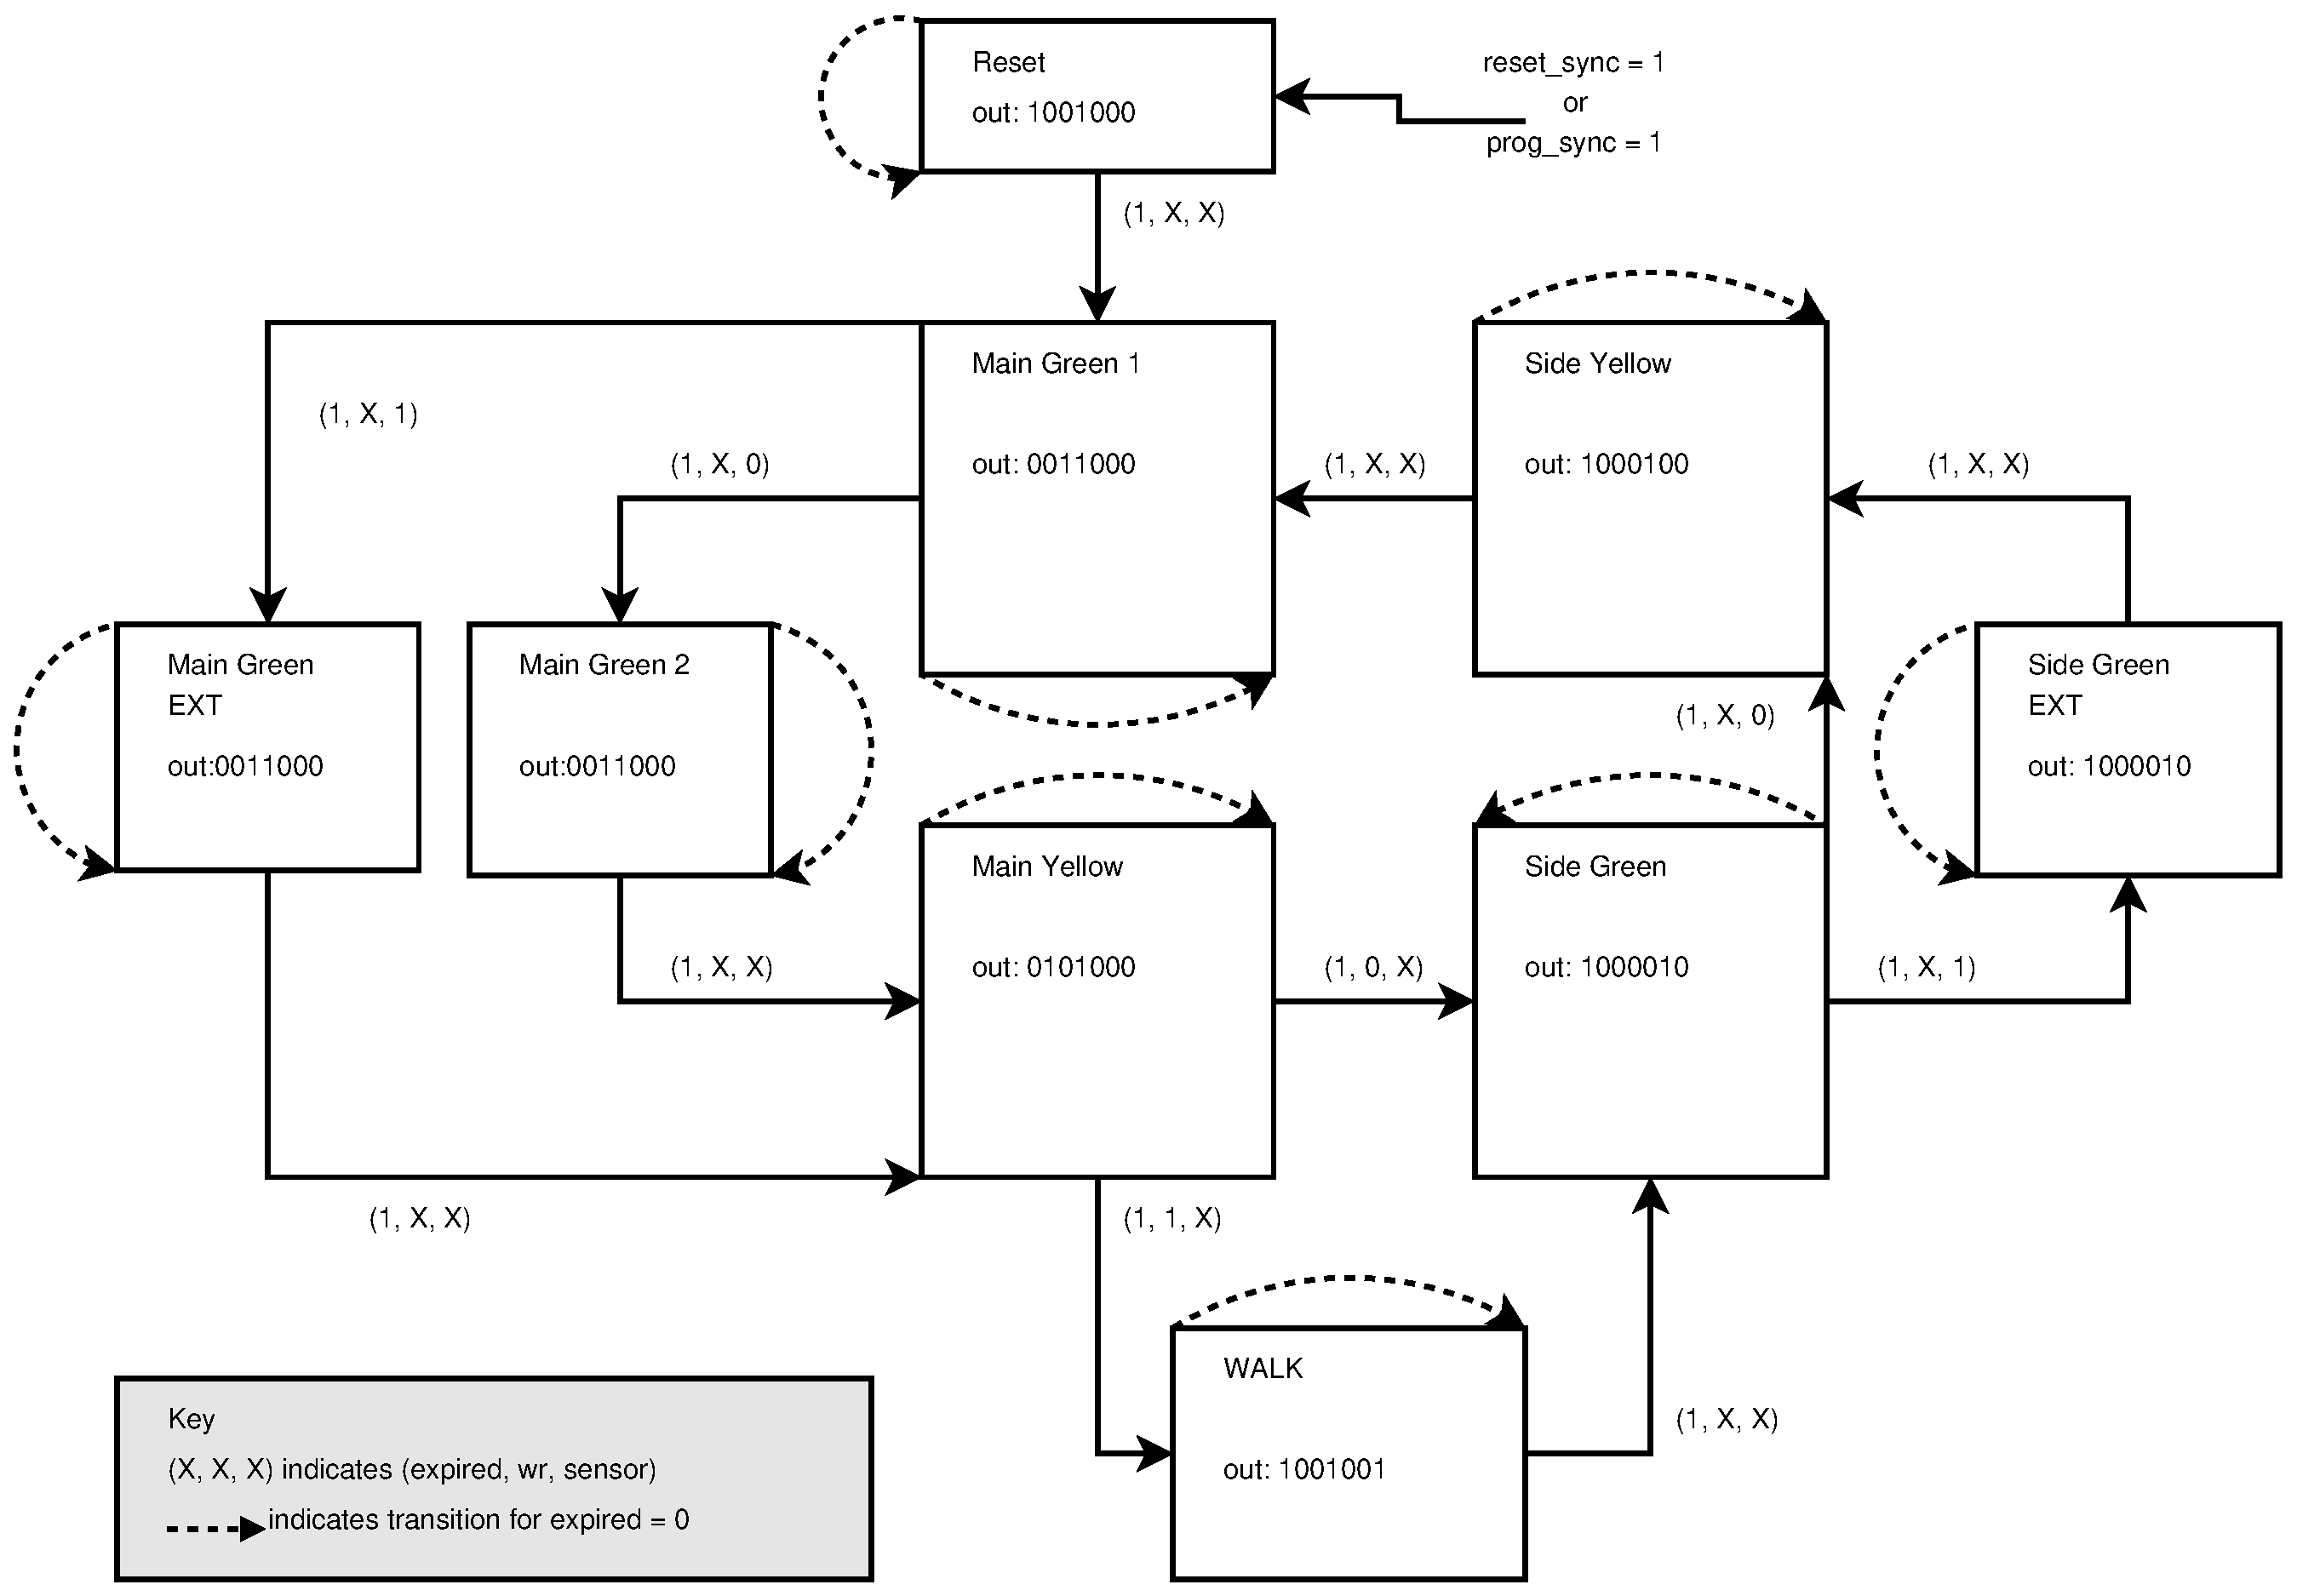
\includegraphics{fsm.ps}
		\caption{Finite State Machine for the Traffic Light Controller}
		\label{fig:fsm}
		\end{figure}
		\end{center}
		Figure~\ref{fig:fsm} shows the finite state machine controlling
		the lights.

\section{Debugging}
	...Was a pain in the ass.

	The most complex interaction was between the FSM, Time Parameter, and
	Timer module.  The MUX was synchronized -- this caused a problem where
	the initial test results reported that there was an off-by-one error
	for the intervals.  The Timer was recieving 'value' signals one clock
	cycle too early.

\section{Conclusions}

\newpage
\section{Appendix: Source Code Listing}
	\subsection{Step to Pulse Module}
		\begin{lgrind}
		\input exsync.v.latex
		\end{lgrind}

	\newpage
	\subsection{Synchronizer}
		\begin{lgrind}
		\input synchronizer.v.latex
		\end{lgrind}

	\newpage
	\subsection{Walk Register}
		\begin{lgrind}
		\input walkregister.v.latex
		\end{lgrind}

	\newpage
	\subsection{Finite State Machine}
		\begin{lgrind}
		\input fsm.v.latex
		\end{lgrind}

	\newpage
	\subsection{Time Parameters}
		\begin{lgrind}
		\input timeparams.v.latex
		\end{lgrind}

	\newpage
	\subsection{Timer}
		\begin{lgrind}
		\input timer.v.latex
		\end{lgrind}

	\newpage
	\subsection{Divider}
		\begin{lgrind}
		\input divider.v.latex
		\end{lgrind}

	\newpage
	\subsection{Top Level Module}
		\begin{lgrind}
		\input controller.v.latex
		\end{lgrind}

\end{document}
